% !Mode:: "TeX:UTF-8"

\chapter[考虑时间缺失值分布特性的填充算法设计]{考虑时间缺失值分布特性的填充算法设计}[考虑时间缺失值分布特性的填充算法设计]
% 15页
\section{引言}
本章主要研究考虑时间缺失值分布特性的填充算法设计。交通数据中的缺失值会改变其时间分布特性,因此,以往的提取时间特征的方法不适用于提取这种带有缺失值的数据的时间特征。为了解决这个问题,本章提出了一种全新的生成式填充神经网络,即多时间流变分自动编码器(\textit{MTS-VAE})。该模型在变分自编码器的基础上,加入了改进的Biconvgrui模块,可以有效提取带有缺失值的交通数据的时间特征。同时,加入改进的双向注意力机制,提高了模型有效区分缺失值和观测值的能力。在三个开源交通数据集上的实验结果显示,本章所提出的填充算法在考虑时间缺失值分布特性的缺失值填充任务上具有优良的填充准确率。

%本章的各节结构如下:\ref{sec3_2}节对问题进行抽象,给出了问题的数学描述;\ref{sec3_3}节介绍所提出的基于时空注意力机制的变分自编码器填充模型,包括模型整体架构和模型训练;\ref{sec3_4}节介绍如何利用时空变分自编码器进行缺失值填充;\ref{sec3_5}节为本章实验及结果分析,包括对比实验和消融实验;\ref{sec3_6}节为本章小结。

\section{问题描述} \label{sec3_2}
考虑时间缺失值分布特性的交通数据缺失问题,本文将一个城市的交通轨迹数据转换为交通流量栅格数据,在每个固定的时间段内,栅格图可视为包含多种通道的图像,那么多个连续的时间段所组成的时空栅格图可视为一段由多个帧按照时间先后顺序堆叠而成的多通道视频流,相关符号的定义如表\ref{tb1}所示。
%\begin{figure}[h]
%\centering
%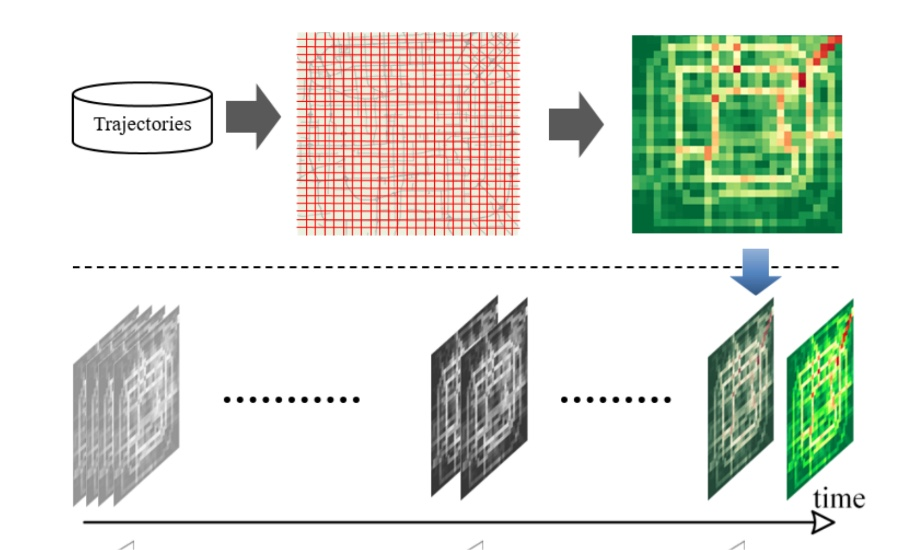
\includegraphics[width = 0.66\textwidth]{video}
%    \vskip 0.2em
%  \wuhao 栅格图中绿色表示该区域上的交通流量较少,红色表示较拥堵。
%    \vspace{0.2em}
%\caption{时空交通流量栅格图 \label{video}}
%\end{figure}

\vspace{1em}
\begin{table}[htbp]
\caption{问题描述中用到的符号定义} \label{tb1}
\vspace{0.5em}\centering\wuhao
\begin{tabular}{ll}
\toprule[1.5pt]
\textbf{符号} & \textbf{定义} \\
\midrule[1pt]
$H$ & 栅格图的高度 \\
$W$ & 栅格图的宽度 \\
$C$ & 栅格图的交通度量数,例如包含出入流量两种度量,则$C=2$ \\
$L$ & 时间范围,以小时为单位,例如$L=24$表示一天 \\
$T$ & 时间范围内的等距时间区间数量,例如$T=48$表示将$L$分成48个时间区间 \\
$\mathcal{X}$ & 样本空间 \\
$X$ & 数据集 \\
$N$ & 样本数量 \\
$x_i$ & 第$i$个样本 \\
$x_i^{obs}$ & 样本$i$的可观测部分 \\
$x_i^{mis}$ & 样本$i$的缺失部分 \\
$\mathcal{M}$ & 掩膜张量空间 \\
$M$ & 掩膜张量,用于标识样本某个位置的值是否缺失 \\
$m$ & 掩膜张量中的元素,取值为0或1 \\
\bottomrule[1.5pt]
\end{tabular}
\end{table}

本文将一个城市根据经纬度划分为一个$H \times W$大小的栅格图,每一个格子都表示一个区域;同时,将一天($L=24$)划分为$T$个时间区间(如$T=48$表示一天有48个时间段,每个区间占半小时),记每日的交通流量为一个数据样本$x \in \mathbb{R}^{C\times T \times H \times W}$。

给定由一些独立同分布的时空交通栅格样本组成的集合$\mathbf{X}=\{x_{i}\}_{i=1}^{N}\in \mathcal{X}^{N}$,其中$\mathcal{X}=\mathbb{R}^{C\times T \times H \times W}$。相应地,定义一个掩膜张量集合$\mathbf{M}=\{m_{i}\}_{i=1}^{N}\in \mathcal{M}^{N}$,其中$\mathcal{M}=\{0,1\}^{C\times T \times H \times W}$,并且如果$x_i[c, t, h, w]$是缺失的,则$m_i[c, t, h, w]=0$;否则$m_i[c, t, h, w]=1$。样本$x_i$中的可观测部分用$x_i^{obs}$表示,缺失部分用$x_i^{mis}$表示。

考虑时间缺失值分布特性的数据填充任务的目标是对于每一个样本$x$,利用观测部分$x^{obs}$的信息填充缺失部分$x^{mis}$,使填充后的值与真实值尽可能地接近。

\section{基于时空注意力机制的变分自编码器填充模型} \label{sec3_3}

\subsection{模型架构}
\begin{figure*}[b]
\vspace{-0.2cm} 
\centerline{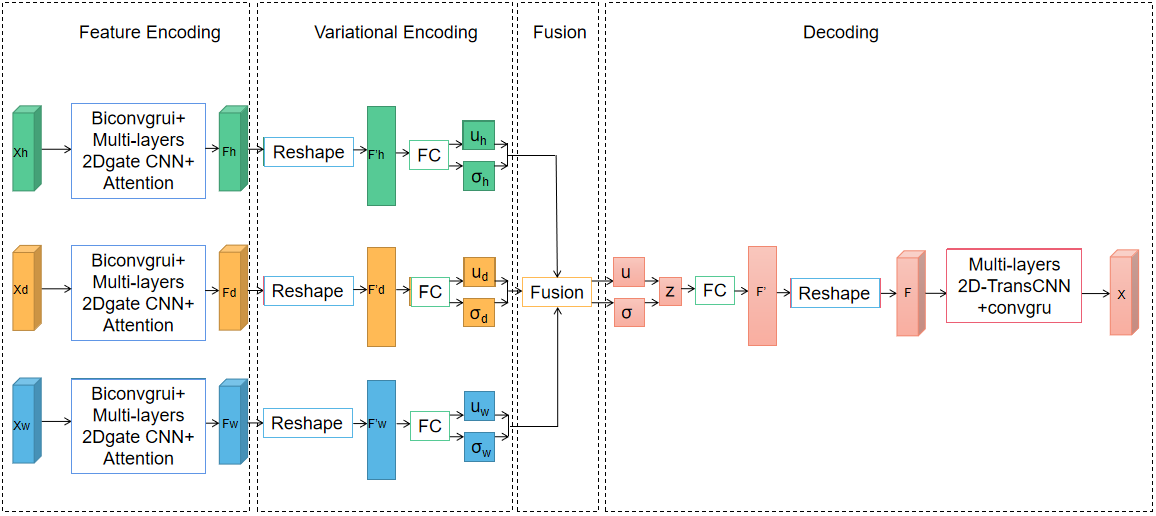
\includegraphics[scale=0.4]{mtsvae.png}}
\caption{多时间流变分自动编码器的整体架构图 \label{MTSVAE}}
\label{fig}
\vspace{-0.2cm} 
\end{figure*}

在本文中,交通数据将被按照不同时间间隔(例如,每小时、每天和每周)划分视频数据研究交通数据填充问题。其中,本文应用了三个时间流数据,包括小时周期、日周期和周周期。每种类型的时间流数据都按照一定的规则进行划分。例如,每小时采样次,取长度为$T_h$, $T_d$ 和 $T_w$的三段,分别作为小时周期、日周期和周周期的输入。因此,可以将小时周期时间流视为张量$x_h \in \mathbb{R}^{C\times T_h\times H\times W}(T_h = \mathcal{P})$,将日周期时间流视为张量$x_d \in \mathbb{R}^{C\times T_d\times H\times W}(T_d = 24\times \mathcal{P})$,将周周期时间流视为张量$x_w \in \mathbb{R}^{C\times T_w\times H\times W}(T_w = 7\times24\times \mathcal{P})$。同时,这些缺失值最初用零填充,这些填充值可以通过\textit{BiConvGRUI}的卷积进行平滑处理。并且填充效果几乎不受此操作的影响\cite{17}。

受\cite{1}的启发,本文提出了一种新颖的基于变分自动编码(\textit{VAE})的多时间流变分自动编码器(\textit{MTSVAE}),用于处理交通数据填充问题。\textit{MTSVAE}可用于学习潜在变量的分布,这个特性帮助其在处理不同缺失率的交通数据时表现强鲁棒性。如图 3-1 所示,多时间流变分自动编码器(\textit{MTSVAE})包含四个关键组件:特征编码、变分编码、融合和解码。特征编码、变分编码和融合用于处理多个时间流数据,而解码用于处理融合数据。

\subsection{特征编码}
\begin{figure*}[htbp]
\vspace{-0.2cm} 
\centerline{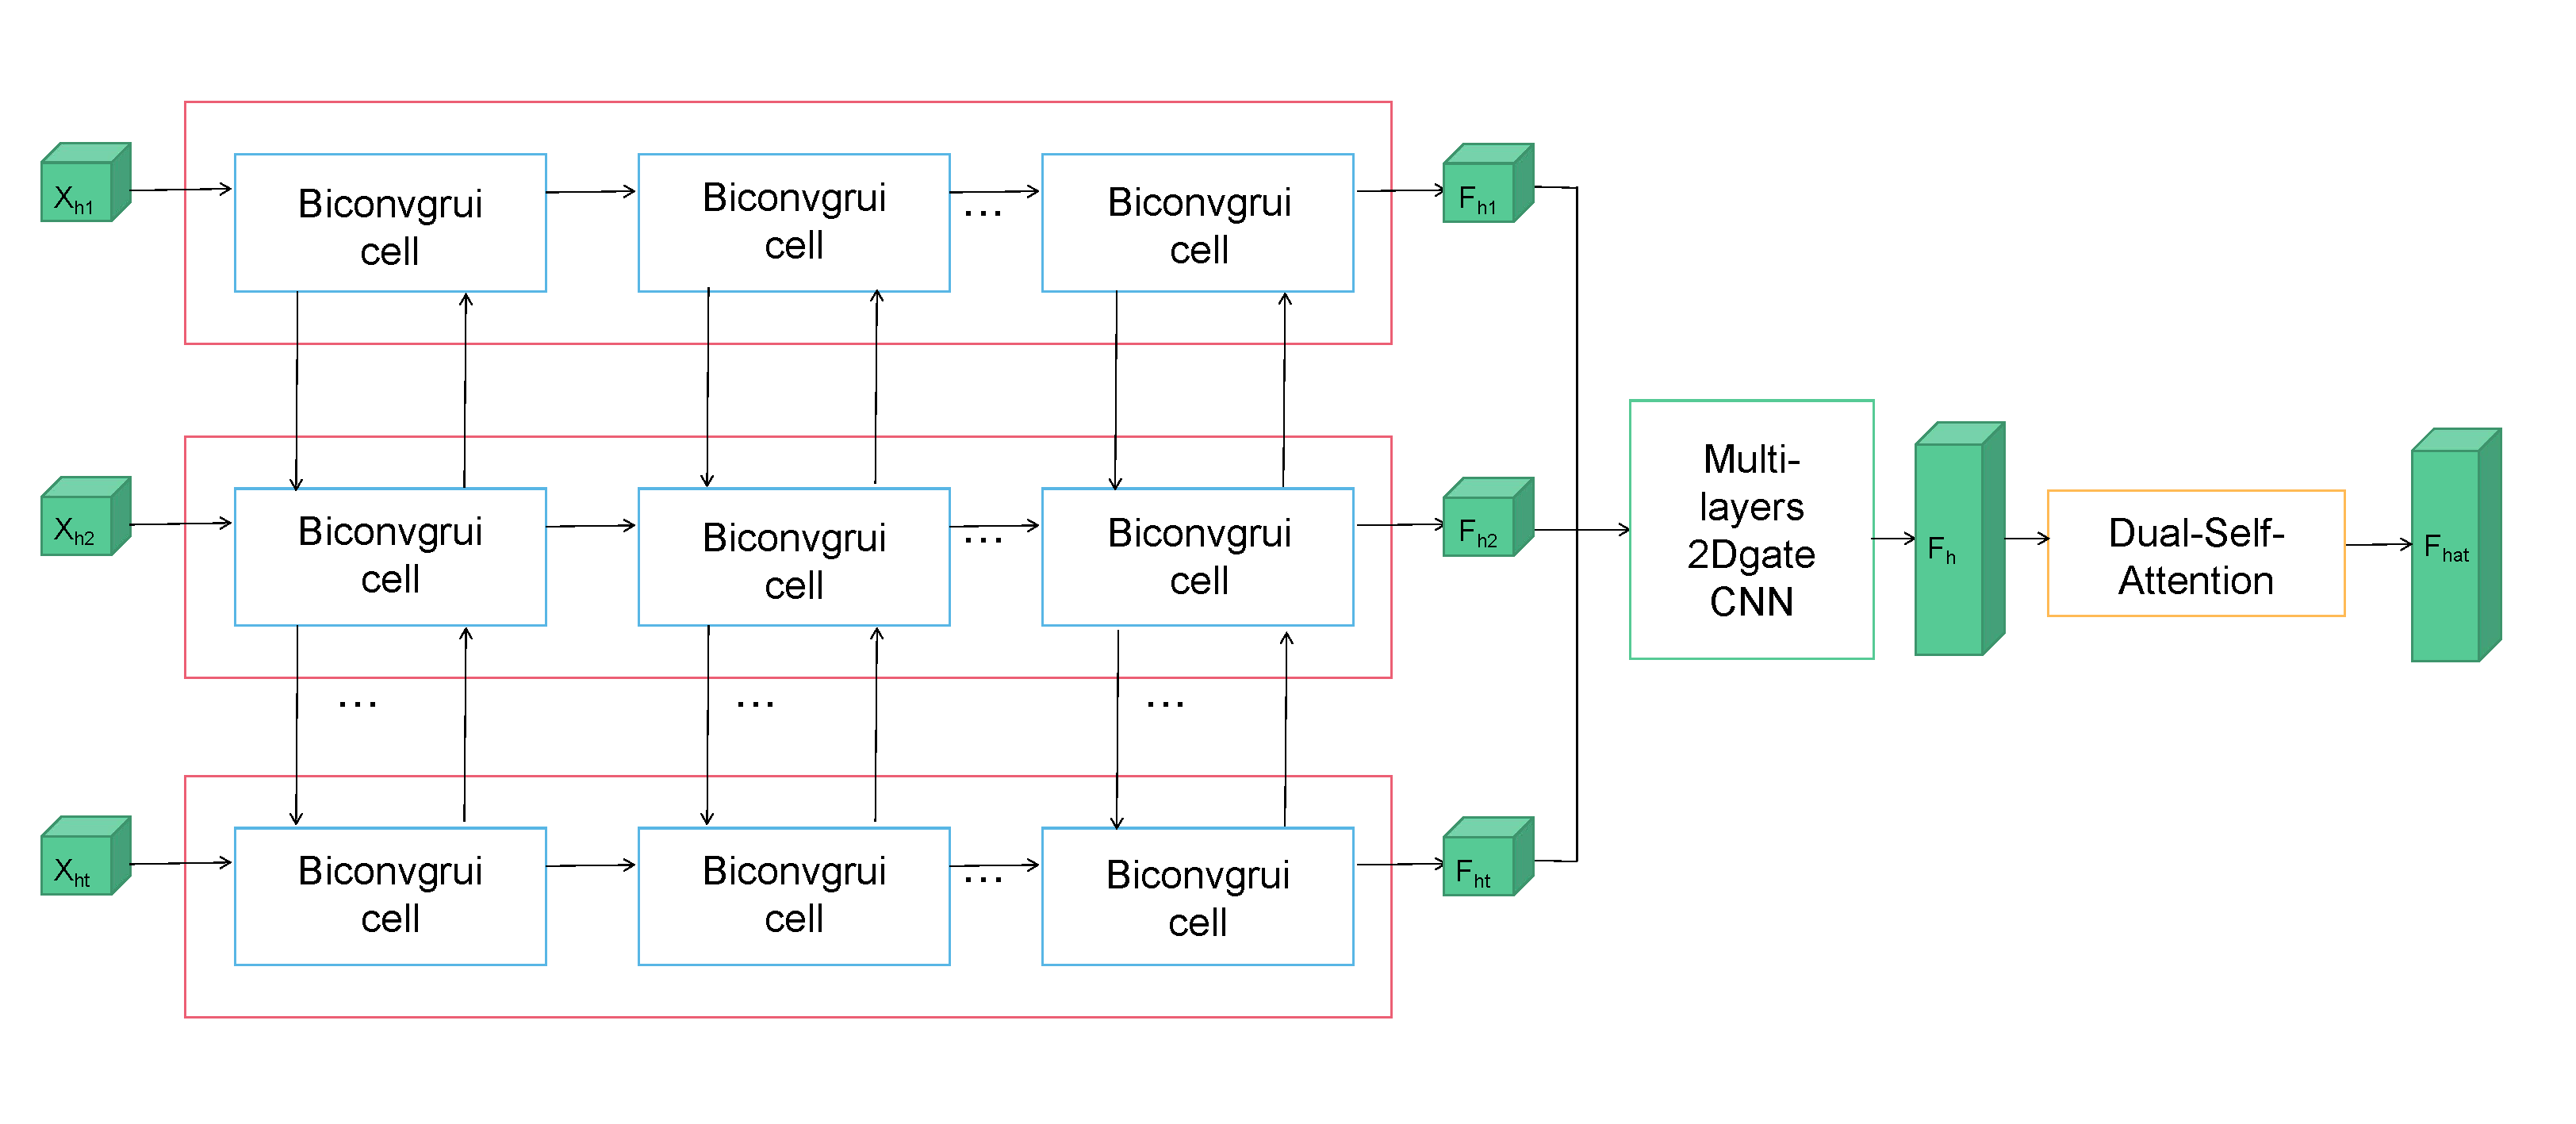
\includegraphics[scale=0.28]{特征编码.pdf}}
\caption{特征编码的整体结构}
\label{fig}
\vspace{-0.2cm}  
\end{figure*}
特征编码模块是\textit{MTSVAE}的一个子模型,它增强了模型捕获不完整数据的时空特征的能力,并使得模型具备区分缺失值与现有值的功能。在特征编码部分中,本章主要设计以下三个模块:1)\textit{BiConvGRUI}模块;2)多层\textit{2D}门控卷积模块;3)双自注意机制模块。如图3-2所示。它们的功能分别是:1)\textit{BiConvGRUI}模块会先刻画带有缺失值的交通数据的时间分布。2)多层\textit{2D}门控卷积被设计来捕获现有值的全局空间特征。3)双自注意机制(由通道自注意力机制和时空自注意力机制组成)被设计以进一步捕捉现有交通数据的动态时空相关性。给定数据$X_d \in \mathbb{R}^{C\times T_d\times H\times W}$作为特征编码的输入,整个特征编码可以用如下公式表示:
\begin{equation}
F_{BI}=B(X_d)
\end{equation}
\begin{equation}
F_{mc}=G(F_{BI})
\end{equation}     
\begin{equation}
F_{att}=M_c(F_{mc})\oplus M_{st}(F_{mc}) 
\end{equation}
其中$F_{BI}\in \mathcal{R}^{C'\times T\times H\times W}$是\textit{BiConvGRUI}的输出特征,$F_{att}\in \mathcal{R}^{C'\times T\times H\times W}$是双自注意力机制的输出特征,$F_{mc}\in \mathcal{R}^{C'\times T\times H\times W}$是多层\textit{2D}门控卷积的输出特征,$\oplus$表示矩阵加法乘积。接下来的内容将分别详细介绍\textit{BiConvGRUI},多层\textit{2D}门控卷积和双自注意力机制。
1)\textit{BiConvGRUI}:\textit{GRUI}在\cite{14}中被提出来并用于多元时间序列的填充问题。\textit{ConvGRUI}\cite{12}与\textit{GRUI}的主要不同是\textit{ConvGRUI}中使用卷积操作替换了\textit{GRUI}中的线性层函数操作,因而\textit{ConvGRUI}适用于处理时空数据。但是,在提取时空数据当前状态的特征时,\textit{ConvGRUI}只关注当前状态之前的时间段信息,而忽略当前状态之后的时间段信息。因此,本章节提出了模型\textit{BiConvGRUI},该模型可以对带有缺失值的交通数据的复杂时间分布进行建模,并捕获当前状态之前和之后的周期信息。与\textit{GRUI}类似,通过提取带有缺失值的交通数据的复杂时间分布特征,\textit{BiConvGRUI}解决了带有缺失值的交通数据的时间特征提取问题。如图3-3所示,\textit{BiConvGRUI}由两个方向相反的\textit{ConvGRUI}组成,分别命名为前向\textit{ConvGRUI}和后向\textit{ConvGRUI}。 
\begin{figure}[htbp]
\vspace{-0.2cm}
\centerline{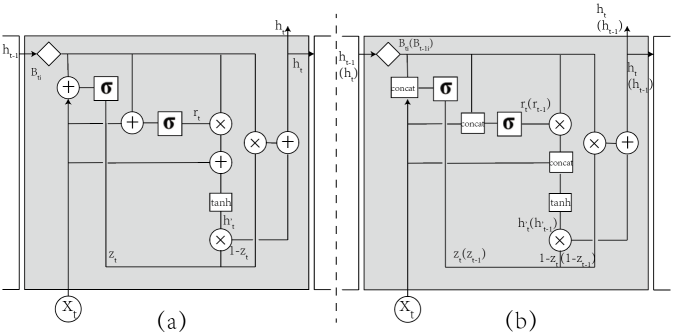
\includegraphics[scale=1.7]{GRUI.png}}
\caption{(a) GRUI和 (b) BiconvGRUI的前向单元(BiconvGRUI的后向单元)}
\label{fig}
\vspace{-0.2cm}
\end{figure}  
 
在\cite{14}中,捕获带有缺失值的数据的时间特征是不容易的。为了捕捉更好的时间特征,本章在模型\textit{BiConvGRUI}中引入了一个新的系数张量$\beta$。系数张量$\beta$可以通过给隐藏状态$h_{t_{i-1}}$中的值进行赋权值,使得模型\textit{BiConvGRUI}处理得到的特征中包含更多的有效特征,进而降低缺失值对于模型\textit{BiConvGRUI}提取时空特征的影响。首先,通过乘以系数张量来更新隐藏状态$h_{t_{i-1}}$:    
\begin{equation}
h'_{pt_{i-1}}={\beta}_{pt_i}\odot h_{pt_{i-1}}
\end{equation}
然后,前向\textit{ConvGRUI}的更新函数为:
\begin{equation}
{\mu}_{pt}={\sigma}(W_{\mu}[h'_{pt_{i-1}},x'_{pt}]+b_{\mu})
\end{equation}
\begin{equation}
r_{pt}={\sigma}(W_r[h'_{pt_{i-1}},x'_{pt}]+b_r)
\end{equation}
\begin{equation}
\tilde{h}_{pt_i}=tanh(W_{\tilde{h}}[r_{pt_i}\odot h'_{pt_{i-1}},x'_{pt}]+b_{\tilde{h}})
\end{equation}
\begin{equation}
{h}_{pt_i}=(1-{\mu}_{pt_i})\odot h'_{pt_{i-1}}+{\mu}\odot \tilde{h}_{pt_i}
\end{equation}
其中$\mu$是更新门系数,$r$是重置门系数,$M_{t_i}$是掩码张量,$\tilde{h}$是候选隐藏状态,$\sigma$是2D卷积函数,[]是拼接操作,$\odot$是逐元素乘法操作,$W_{\mu}$, $W_t$, $W_{\tilde{h}}$, $b_{\mu}$, $b_r$, $b_{\tilde{h}}$和$b_H$是需要训练的参数。后向\textit{ConvGRUI}的更新函数类似于前向\textit{ConvGRUI}的更新函数。而后向\textit{ConvGRUI}被用于提取未来时间的信息。相反,前向\textit{ConvGRUI}被用于提取过去时间的信息。
最后,将前向时间特征$h_{pt_i}$和后向时间特征$h_{ft_i}$融合为时间特征$H_{t_i}$:
\begin{equation}
H_{t_i}=tanh(W_y^{\overset{\rightarrow}{h}}*h_{pt_i}+W_y^{\overset{\leftarrow}{h}}*h_{ft_i}+b_H) 
\end{equation}
其中 ,$W_y^{\overset{\rightarrow}{h}}$, $W_y^{\overset{\leftarrow}{h}}$是训练参数。
在\textit{BiConvGRUI}中,系数张量$\beta$需要找寻到一个适当的权重矩阵,使得隐藏状态的值能够包含更多的有效信息。并且系数张量$\beta$的值需要落在(0, 1)的范围内。参考原论文\cite{14},的计算方式如下:
\begin{equation}
{\beta}_{t_i}=1/e^{[max(0,W_{{\beta}}{\delta}_{t_i}+b_{{\beta}})]}
\end{equation}
其中$W_{{\beta}}$和$b_{{\beta}}$是需要学习的参数。

为了捕捉更好的时间信息,本课题引入了一个可学习的参数${\theta}$(${\theta}$最初设置为0.8),它可以被用来扩展$max(0,W_{{\beta}}{\delta}_{t_i}+b_{{\beta}})$的取值范围,以帮助模型找到更合适的值。前向\textit{ConvGRUI}的计算方式如下:
\begin{equation}
{\beta}_{pt_i}=1/e^{[max(0,W_{{\beta}_p}{\delta}_{pt_i}+b_{{\beta}_p})]^{\theta}}
\end{equation}                                              
此外,使用\textit{ReLU}激活函数计算\textit{max}的结果。后向\textit{ConvGRUI}的计算方式如下:
\begin{equation}
{\beta}_{ft_i}=1/e^{[max(0,W_{{\beta}_f}{\delta}_{ft_i}+b_{{\beta}_f})]^{\theta}}
\end{equation}
为了得到准确的系数张量$\beta$,本章将进一步引入时间滞后张量$\delta$。时滞是指将有用信息从前一时刻传递到当前时刻所需的时间。并且可以通过当前时刻与前一时刻之间的差异来计算时滞。通过记录当前值和最后一个有效值之间的时间滞后值,就可以标记缺失值附近的值,以获得准确的系数张量$\beta$。对于前向\textit{ConvGRUI},我们可以设置当前时刻与前一时刻的差为1。因此,当前一时刻的值存在时,对应的时滞设置为1。当前一个时刻的值丢失时,就没有从前一个时刻传递到当前时刻的任何有效信息。然后,将这个时滞的值设置为前一个时滞的值加 1(即当前时刻与前一时刻的差值)。因此,前向\textit{ConvGRUI}的时滞张量计算公式如下: 
\begin{equation}
{\delta}_{pt_i}^{c\times h\times w}=\begin{cases}
1,&\mathcal{M}_{pt_{i-1}}^{c\times h\times w}==1\\
{\delta}_{pt_{i-1}}^{c\times h\times w}+1,&\mathcal{M}_{pt_{i-1}}^{c\times h\times w}==0 and i>0\\
0,&i==0
\end{cases}
\end{equation}
其中,$pt_i$, $pt_{i-1}$分别代表相邻的两个时间点,$\mathcal{M}_{pt_{i-1}}^{c\times h\times w}$表示在时间点坐标 (c,h,w) 对应的值是否缺失,缺失时为0,否则为1。
对于后向的\textit{ConvGRUI},本课题将当前时刻与上一个时刻的差值设置为 -1。而后向\textit{ConvGRUI}的时滞张量计算公式如下:
\begin{equation}
{\delta}_{ft_i}^{c\times h\times w}=\begin{cases}
-1,&\mathcal{M}_{ft_{i-1}}^{c\times h\times w}==1\\
{\delta}_{ft_{i-1}}^{c\times h\times w}-1,&\mathcal{M}_{ft_{i-1}}^{c\times h\times w}==0 and i>0\\
0,&i==0
\end{cases}
\end{equation}
其中,$ft_i$, $ft_{i-1}$分别代表相邻的两个时间点。
在栅格地图的区域中,观察到的时间序列作为样本给出:
\begin{equation}
X= \begin{bmatrix}
none & 9 & none & 4\\
2 & none & 5 & none\\
3 & none & none & 9\nonumber
\end{bmatrix}
T= \begin{bmatrix}
0\\
1\\
2\nonumber
\end{bmatrix}
\end{equation}
其中“none”是缺失值。根据公式(2-13)和(2-14),可以得到两个时滞张量:
\begin{equation}
{\delta}_{pt_i}= \begin{bmatrix}
0 & 0 & 0 & 0\\
1 & 1 & 1 & 1\\
1 & 2 & 1 & 2\nonumber
\end{bmatrix}
{\delta}_{ft_i}= \begin{bmatrix}
0 & 0 & 0 & 0\\
-1 & -1 & -1 & -1\\
-1 & -2 & -1 & -2\nonumber
\end{bmatrix}
\end{equation}
2)多层 \textit{2D} 门控卷积:在\cite{10}中,\textit{2D}门控卷积由于在普通卷积的基础上加入了门机制,使得相比起普通卷积,它更适用于图像修复问题。在本章中,\textit{2D}门控卷积将被用于交通数据填充问题。同时,由于\textit{2D}门控卷积较好的提取空间特征的性能,可以显著增强模型提取空间特征的能力。与\textit{2D}卷积类似,由于卷积核大小的限制,会限制模型卷积的范围。因此,在编码模块中堆叠了多个\textit{2D}门控卷积,命名为多层\textit{2D}门控卷积,以扩大卷积的范围,从而使得模型可以学习全局特征。在每个时间间隔中,\textit{2D}门控卷积最初检测哪些像素包含无效消息(即先前缺失的部分),并更加关注有效消息以学习重要特征。

3)双自注意力机制:双注意力机制\cite{15}被提出用于场景分割。然而,原始双注意力机制只关注空间数据。在本章中,使用在双注意力机制基础上扩展的双自注意力机制机制来处理时空问题。它由通道自注意力机制和时空自注意力机制组成,如图3-4和图3-5所示。而且时空自注意力和通道自注意力从输入特征中并行学习目标的相关特征。最后将它们各自的输出相加作为最终输出。具体说明如下:

时空自注意力机制。与双注意力机制的空间自注意力不同,时空自注意力机制可以处理时空数据。把特征$F_{mc}\in \mathbb{R}^{C'\times T\times H\times W}$作为时空自注意力的输入。首先,特征经过卷积操作和重构操作可以得到特征图$F’_{mc}\in \mathbb{R}^{C'\times N}$。然后,将特征$F’_{mc}$同$F’_{mc}$的转置进行乘积操作,经过softmax激活函数的操作,生成权重分布矩阵$F''_{mc}\in \mathbb{R}^{N\times N}$。最后将特征$F’_{mc}$与权重分布矩阵$F''_{mc}$相乘,并将输出重塑为与特征$F_{mc}$相同的形状,这样就可以将多个特征相加生成特征$F_{st}$。
\begin{figure}[htbp]
\centerline{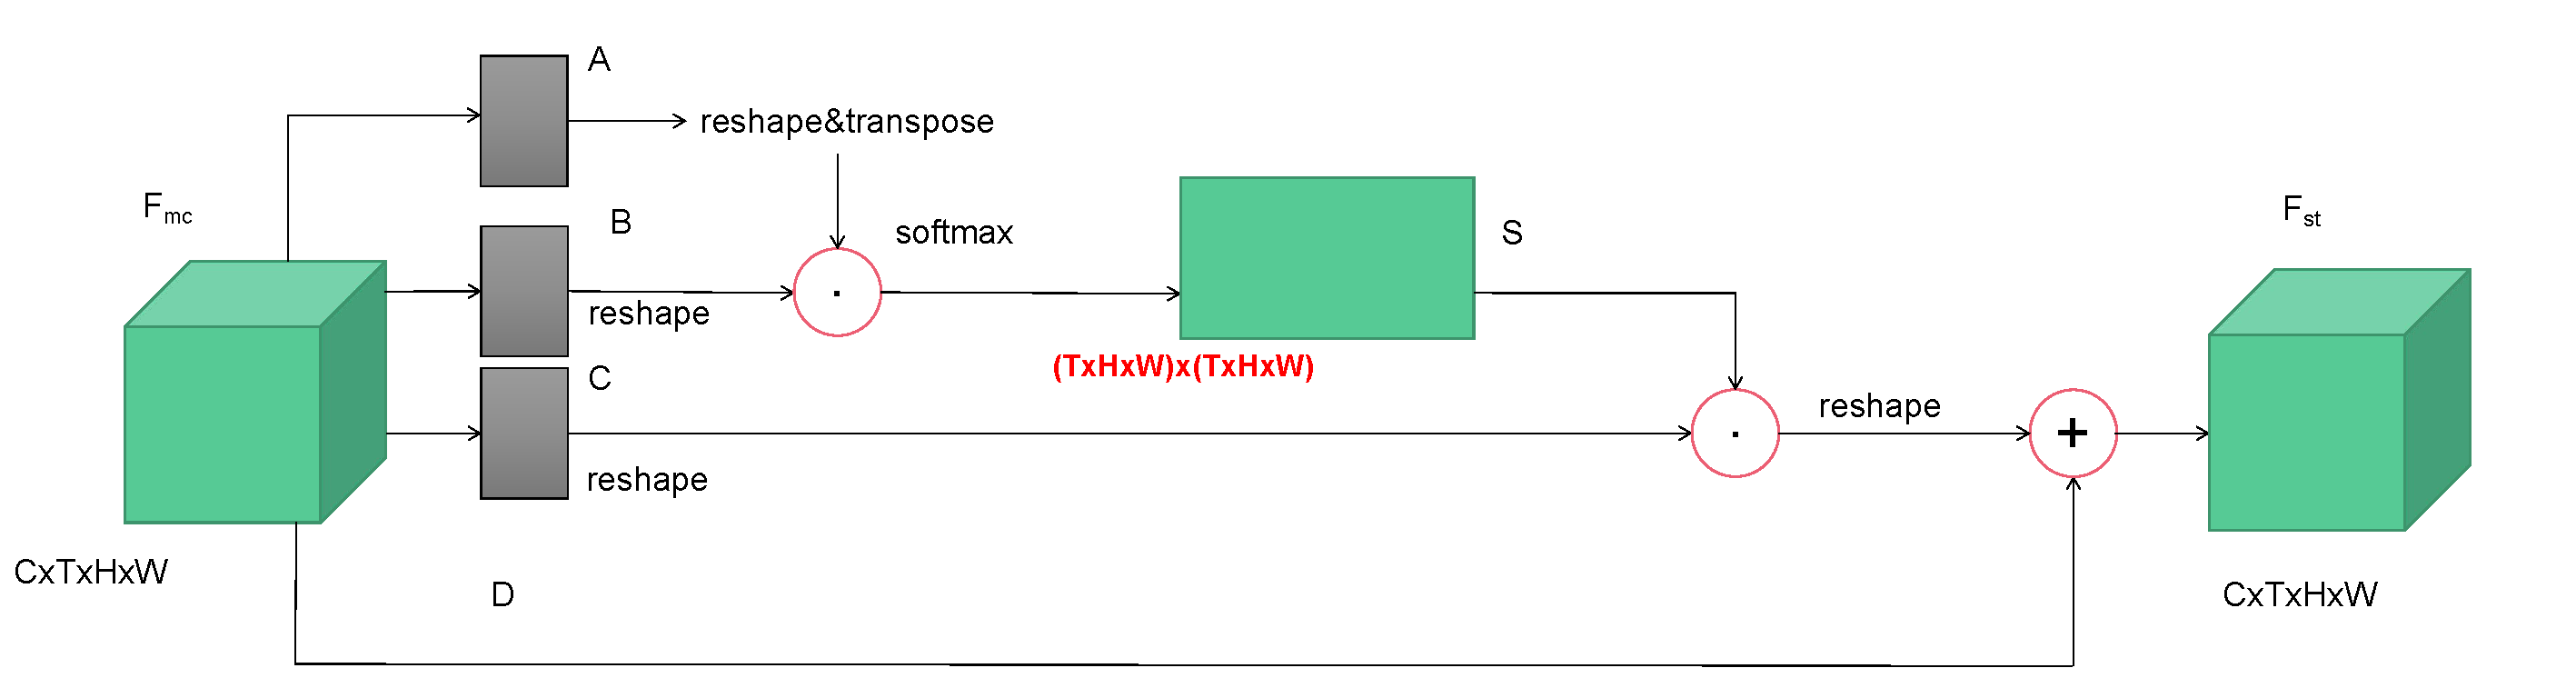
\includegraphics[scale=0.3]{时空自注意力整体结构.pdf}}
\caption{时空自注意力整体结构}
\label{fig}
\end{figure}

通道自注意力机制。在双自注意力机制中,还有一个重要的组成构建-通道自注意力。通道自注意力机制通常被用来学习交通数据的流入和流出的相关性。把特征$F_{mc}\in \mathbb{R}^{C'\times T\times H\times W}$作为通道自注意力的输入。首先,特征$F’_{mc}\in \mathbb{R}^{C'\times N}$经过重塑操作,可以得到三个特征图$F’_{mc}\in \mathbb{R}^{C'\times N}$。然后,将特征$F'_{mc}$乘以$F’_{mc}$的转置,得到的结果通过softmax激活函数的操作生成权重分布矩阵$F''_{mc}\in \mathbb{R}^{C'\times C'}$。最后将特征$F’_{mc}$与权重分布矩阵$F''_{mc}$相乘,并将输出重塑为与特征$F_{mc}$相同的形状,这样就可以将特征$F_{mc}$相加生成特征$F_{st}$。
\begin{figure}[htbp]
\vspace{-0.2cm}
\centerline{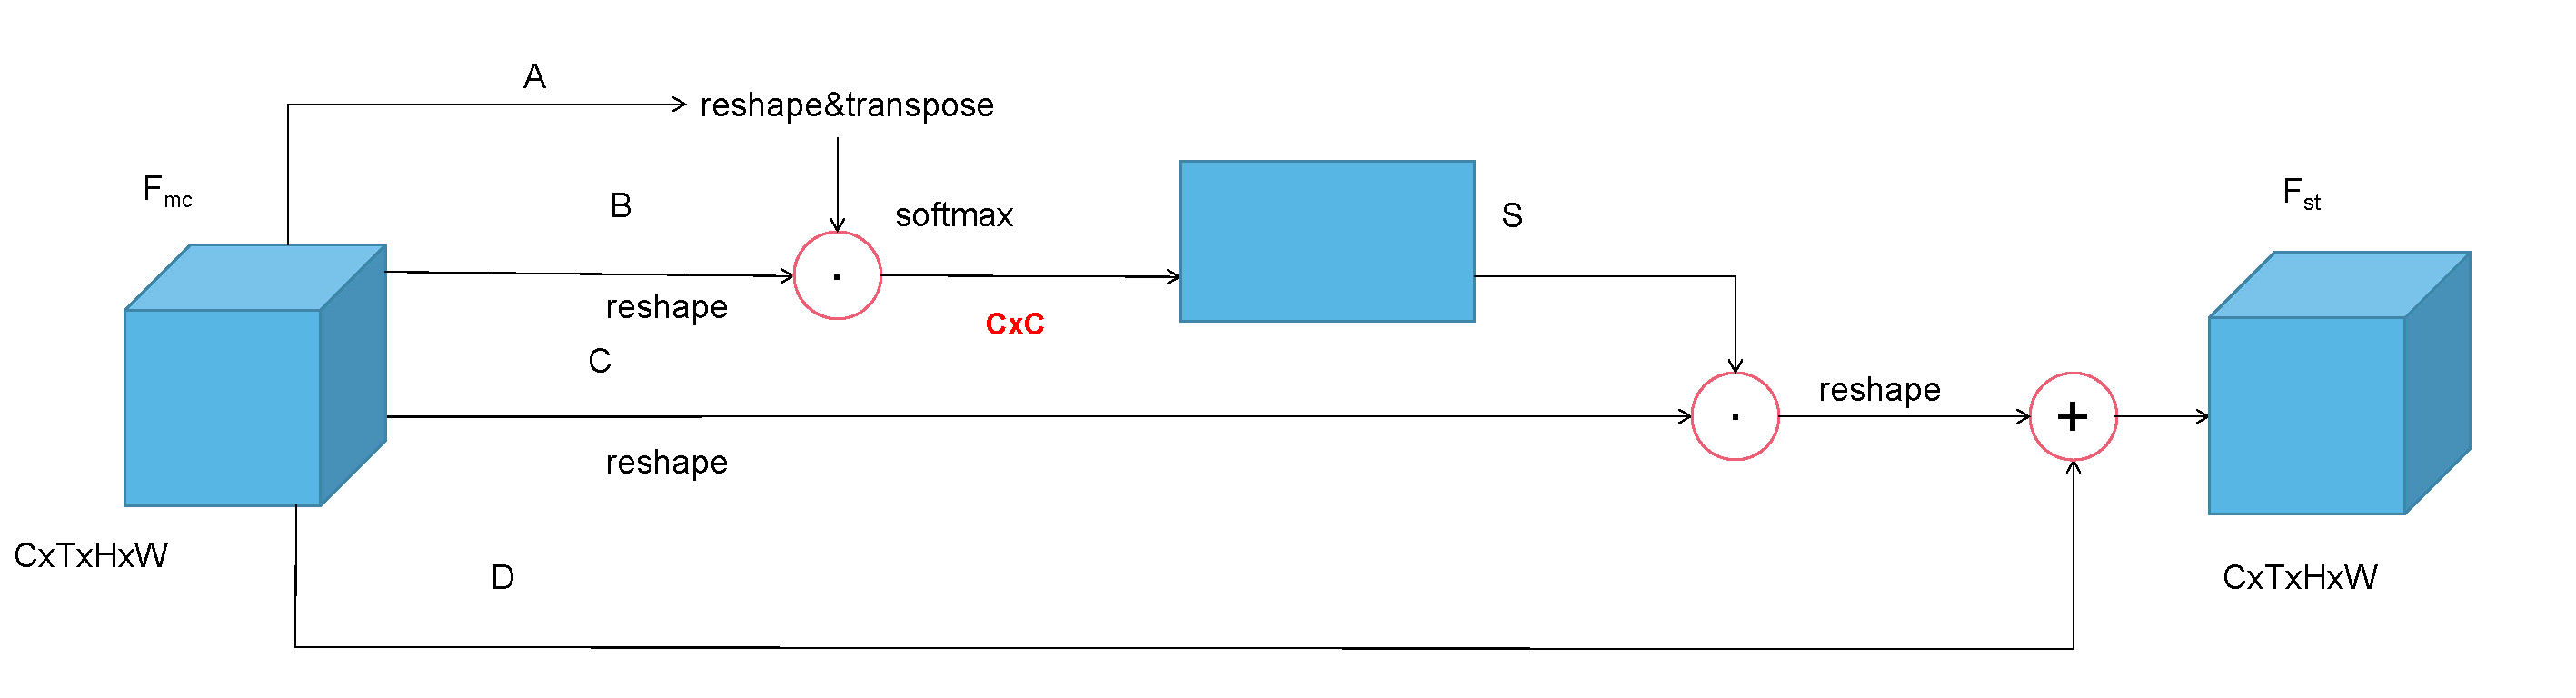
\includegraphics[scale=0.3]{通道自注意力整体结构.pdf}}
\caption{通道自注意力整体结构}
\label{fig}
\vspace{-0.2cm}
\end{figure}

最后将$F_{st}$和$F_{c}$求和为$F_{att}\in \mathbb{R}^{C'\times T\times H\times W}$,如上式(3-3)所示。

\subsection{变分编码}
模型的鲁棒性是衡量模型在存在外界干扰的情况下的性能。这意味着,如果模型的鲁棒性越强,那么它抗干扰的能力也就越强。而在本文中,定义的外界干扰主要是指交通数据中存在的缺失值。因而,如何使模型呈现更好的鲁棒性,抵御这种外界干扰,是一个很重要的问题。在VAE\cite{18}算法中,通过在编码过程中引入高斯噪声,可以提高模型的鲁棒性。这种编码过程被称为变分编码。同时,引入高斯噪声可以帮助模型捕获更多有效信息。受此启发,本章决定应用变分编码来增强模型的鲁棒性。在变分编码过程中,输入经过扁平层和线性层的处理,生成初始潜变量$z$的参数化均值$\mu$和对数偏差$log{\sigma}^2$。接下来,可以通过重新参数化技巧\cite{16}生成$z$,如下所示:

\begin{equation}
z=\mu+\sigma\oplus\varepsilon
\end{equation}  
其中${\mu}$是从$\mathit{N}(0,1)$中采样的, $\oplus$是矩阵加法。
\subsection{融合}
在融合模块中,三个相互独立的分布函数可以通过加权融合形成一个新的分布函数。$\mu$和$\sigma$可以分别表示为:
\begin{equation}
{\mu}_k=w_h\otimes {\mu}_h+w_d\otimes {\mu}_d+w_w\otimes {\mu}_w
\end{equation}
\begin{equation}
{\sigma}_k^2=w_h\otimes {\sigma}_h^2+w_d\otimes {\sigma}_d^2+w_w\otimes {\sigma}_w^2
\end{equation}
其中,$w_h$, $w_d$, $w_w$是需要在训练过程中学习的参数,数值表示每个独立时间分量对最终结果的影响程度。$\otimes$是\textit{Hadamard}乘积。
\subsection{解码}
解码模块用于重构样本。其中解码模块由四个部分组成,分别称为压缩层、重塑层、多层2D反卷积和convGRU。其中,多层2D反卷积用于重构空间信息,convGRU用于重构时间信息。给定融合模块的输出作为解码模块的输入,使用压缩层和重塑层从融合的潜在变量中重构时空特征。然后,重建的时空特征被输入到多层2D反卷积中进行处理,再将处理结果通过convGRU重建完整的交通数据$X_k$。用公式(3-19)训练$X_k$。在损失函数收敛到最优解后,应用$X_k$的值来替换$X$的缺失值,如下所示:

\begin{equation}
X_{imputation}=M\odot X+(1-M)\odot X_k
\end{equation}

\section{模型训练}
在普通的VAE的损失函数基础上,将KL损失函数中的普通高斯分布替换为融合高斯分布,得到MTSVAE的损失函数,结果如式(3-19)所示。  
\begin{align}
&\mathcal{F}=\sum_{i=1}^{T}m_i\otimes||x_i-\bar{x}_i||_F\\
&+\beta\sum_{i=1}^{T}KL \Big(N(w_{hi}\otimes{\mu}_{hi}+w_{di}\otimes{\mu}_{di}+w_{wi}\otimes{\mu}_{wi},\nonumber\\
&w_{hi}\otimes{\sigma}_{hi}^2+w_{di}\otimes{\sigma}_{di}^2+w_{wi}\otimes{\sigma}_{wi}^2)||N(0,1) \Big)\nonumber
\end{align}
式(3-19)中,$\beta$为超参数,用于平衡两部分的损失,$\otimes$为Hadamard乘积。由于缺乏完整的数据集,第一项需要计算为$m_i\otimes||x_i-\bar{x}_i||_F$,表示观察部分$x_i^{obs}$的重建误差。最后一项是两个分布之间的\textit{Kullback-Leibler}距离。(即潜在变量的分布$N(w_{hi}\otimes{\mu}_{hi}+w_{di}\otimes{\mu}_{di}+w_{wi}\otimes{\mu}_{wi},w_{hi}\otimes{\sigma}_{hi}^2+w_{di}\otimes{\sigma}_{di}^2+w_{wi}\otimes{\sigma}_{wi}^2)$和目标分布$N(0,1)$)。
\begin{figure}[htbp] 
\centering
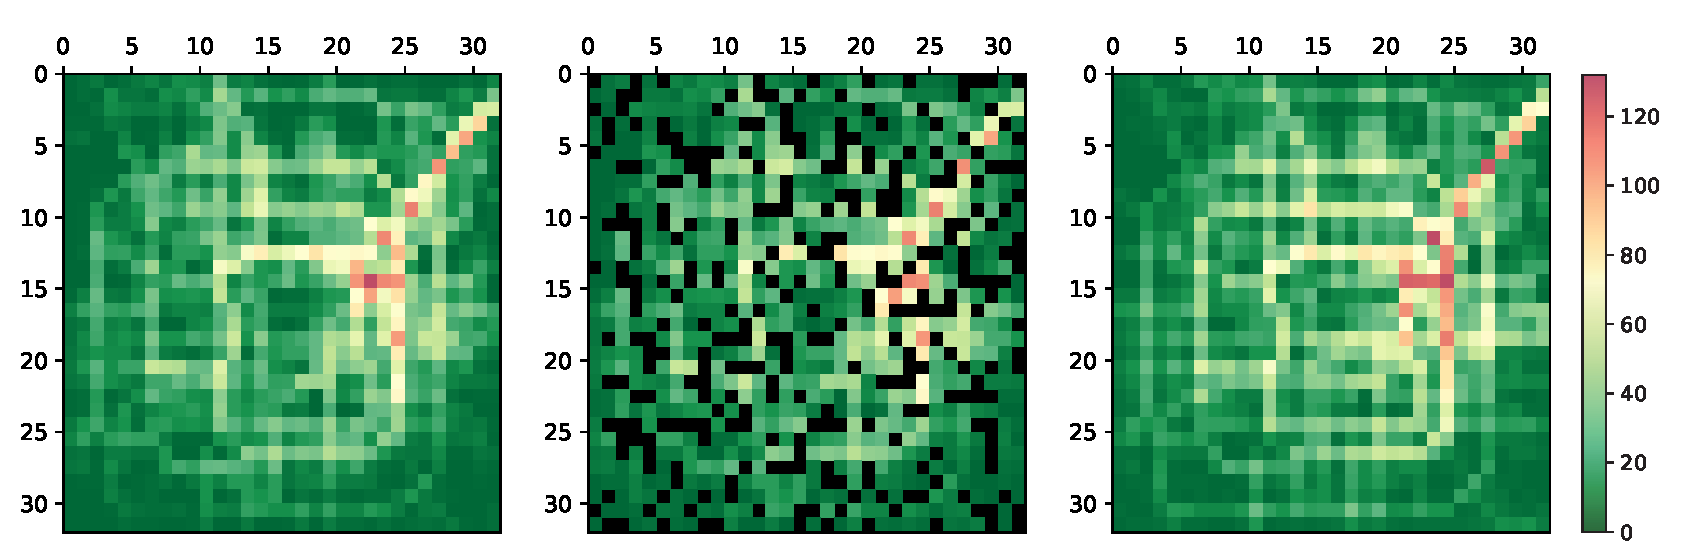
\includegraphics[width=\textwidth]{impute.eps}
\vspace{-1em}
\caption{填充效果图 \label{impute}}
\end{figure}
\section{模型推断}
一旦模型训练完毕, MSTVAE 可以被用于重构缺失值, 公式如下所示:
\begin{equation}
p(x^{mis}|x^{obs}) = \int p_{\theta}(x^{mis}|z_{K})q_{\phi}(z_{K}|x^{obs}) dz_{K},	
\end{equation}

即可以在给定数据的观测值的条件下推断出其缺失部分,其中最主要的就是借助隐变量作为推断的桥梁。本文选取了TaxiBJ数据集中某一时刻的交通梜格数据作为填充效果的展示,如图3-7所示,绿色表示该区域上的交通人流量较少,红色表示人流量较多。左边的图表示真实的栅格数据,中间的图由真实数据根据MCAR模式随机缺失产生,右边的图为缺失数据经过本文模型处理后得到的完整数据。左右两幅图差异越小表明模型填充效果越好。

\section{实验与分析}
本小节首先介绍了实验所用的数据集,然后列出了实验环境和模型参数的设置,接着进行了对比实验和模型复杂度的分析,最后给出了消融实验的结果。
\subsection{数据集}
为了定量地评价所提出的模型的填充效果,本文在如下三个开源的交通轨迹数据集上做了对比实验,分别为TaxiBJ\cite{zhang2017deep}、TaxiNYC\cite{illinoisdatabankIDB-9610843}、BikeNYC\cite{zhang2017deep},数据集概况如表\ref{tb_dataset}所示。

(1)\textbf{TaxiBJ:}该数据集为北京市内所有出租车GPS轨迹数据,分别从四个时间段进行记录:2013年7月1日至2013年10月30日、2014年3月1日至2014年6月30日、2015年3月1日至2015年6月30日、2015年11月1日至2016年4月10日。

(2)\textbf{TaxiNYC:}该数据集包含了从2010年到2013年间纽约市的出租车GPS记录,其中有近70亿条出租车接送客轨迹数据,每个记录包括了接送客的具体时间戳、位置坐标和行驶距离。

(3)\textbf{BikeNYC:}该数据集来自纽约市自行车租赁系统,日期从2014年4月1日至2014年9月30日。每一条轨迹数据包括租赁开始时间戳、结束时间戳、租赁时长、起始租赁点和归还点ID。

以上轨迹数据均可通过定义(\ref{def_flow})转换为交通出入流量数据。本文按照五个缺失值比例10\%,30\%,50\%,70\%,90\%随机手动生成相应的数据集,接着使用归一化将数据集数值范围缩放到区间[-1,1]内。对于每个数据集,本文将数据集前90\%的样本作为训练集,剩余的样本作为测试集,又取训练集中的90\%作为验证集。为了防止模型训练产生过拟合现象,我们保存在验证集上损失函数最小的模型参数用于测试。


\begin{table}[htbp] 
\renewcommand\arraystretch{1.2}
\caption{数据集描述} \label{tb_dataset}
\vspace{0.5em}\centering\wuhao
\begin{tabular*}{\hsize}{@{}@{\extracolsep{\fill}}cccc@{}}
\toprule[1.5pt]
数据集 & TaxiBJ\cite{zhang2017deep} & TaxiNYC\cite{illinoisdatabankIDB-9610843} & BikeNYC\cite{zhang2017deep} \\
\midrule[1pt]
数据类型 & 出租车GPS        & 出租车GPS         & 自行车租赁 \\ 
采集地点 & 北京 & 纽约 & 纽约\\
时间范围 & \makecell[c]{7/1/2013 $\sim$ 10/30/2013\\3/1/2014 $\sim$ 6/30/2014\\3/1/2015 $\sim$ 6/30/2015\\11/1/2015 $\sim$ 4/10/2016} & \makecell[c]{1/1/2010 $\sim$ 12/31/2010\\1/1/2012 $\sim$ 12/31/2013} & \makecell[c]{4/1/2014 $\sim$ 9/30/2014} \\ 
时间区间 & 30 分钟      & 1 小时   & 1 小时 \\
栅格图尺寸   & (32, 32)        & (10, 20)         & (16, 8) \\
时间区间数 & \num[group-separator={,}]{22459}   & \num[group-separator={,}]{26304}          & 4392 \\
\bottomrule[1.5pt]
\end{tabular*}
\end{table}

\subsection{实验设置}
(1)\textbf{实验环境}:本章实验均在GPU服务器上完成,表\ref{env1}给出了实验所采用的软硬件环境的具体细节。
\begin{table}[htbp] 
\caption{实验软硬件环境} \label{env1}
\vspace{0.5em}\centering\wuhao
\begin{tabular}{cc}
\toprule[1.5pt]
环境 & 参数 \\
\midrule[1pt]
操作系统 & Ubuntu 20.04.2.0 LTS \\
内存 & 128GB \\
磁盘 & 1TB SSD \\
处理器 & 英特尔至强Gold 5218R@2.10GHz \\
图形卡 & GeForce RTX 3080 \\
CUDA版本 & 11.1 \\
开发语言 & Python 3.8 \\
深度学习框架 & Pytorch 1.8.1 \\
\bottomrule[1.5pt]
\end{tabular}
\end{table}

(2)\textbf{模型超参设置}:在BiconvGRUI模块中,我们将内核大小调整为3,步幅调为2,输出通道数调整为16。BiconvGRUI单元格的数量被设置为6(小时流)、24(每日流)和48(周流)。对于每个二维卷积模块,内核大小被调整为3,步幅被调整为2。每个二维卷积的输出通道数按升序依次为32、64和128。在congGRU模块中,我们将内核大小调整为3,步幅调为2,输出通道数调整为2。我们根据经验设置convGRU细胞的数量为24个。利用Adam优化器进行梯度下降,初始学习速率设置为$10^{-3}$。此外,我们还将TaxiNYC、TaxiBJ和BikeNYC的epoch总数分别设置为200、500和2000。

(3)\textbf{评价指标}:为了定量评估本章节的方法和基线方法,通过归一化均方误差(\textit{NMSE})和均方根误差(\textit{RMSE})来衡量真实数据和估算数据的适用性,其定义为
\begin{equation}
NMSE=\frac{1}{t}*\frac{\sum_{j=1}^J\sum_{k=1}^K[(1-M)\otimes(x-\bar{x})]^2}{\sum_{j=1}^J\sum_{k=1}^K[(1-M)\otimes x]^2}
\end{equation}
\begin{equation}
RMSE=\sqrt{\frac{1}{t}*{\sum_{j=1}^J\sum_{k=1}^K[(1-M)\otimes(x-\bar{x})]^2}}
\end{equation}

\subsection{对比实验结果与分析}
在本节中,将模型MTSVAE与九种基线方法进行比较:ARIMA\cite{3}、knn\cite{19}、HaLRTC\cite{4}、ConvLSTM\cite{20}、DeepSTNPlus\cite{5}、CombCN\cite{21}和 ST-VAE\cite{8}。

图3-7至图3-9显示了MTSVAE和其他基线模型在三个不同缺失率数据集上的RMSE和NMSE的比较结果。本章提出的模型MTSVAE在不同缺失率的数据集中都得到最低的RMSE和NMSE,这表明,模型MTSVAE具有较强的鲁棒性,因而相比其它模型,它更适用于处理交通数据的填充问题。

\begin{figure}[htbp] 
\centering
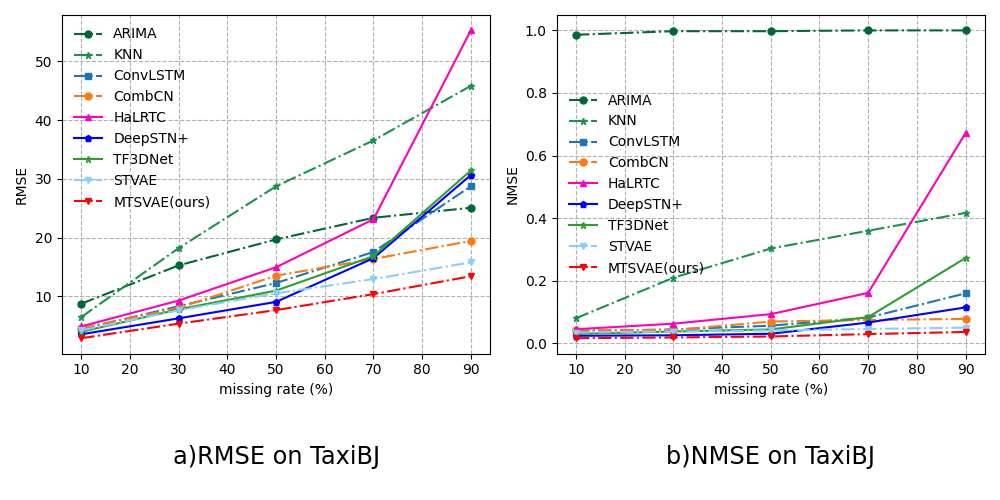
\includegraphics[width=\textwidth]{myplot_taxibj.png}
\vspace{-1em}
\caption{填充效果图 \label{impute}}
\end{figure}

对于传统方法(Auto-Regressive Integrated Moving Average(ARIMA)和 k-NearestNeighbor(KNN)),ARIMA主要关注预测值的历史记录,即时间特征,而忽略了空间特征。相比之下,knn主要关注于空间特征,而忽略了时间特征。对于基于张量的方法(HaLRTC),它同时使用了时间特征和空间特征。因此,由图3-8和图3-9可以发现,HaLRTC应用在缺失率较低的TaxiNYC和BikeNYC两个数据集上时,其表现结果都优于ARIMA和KNN。但它只利用了短期历史特征和局部空间特征,而忽略了长期历史特征和全局空间特征,限制了HaLRTC在TaxiBJ数据集中的结果。相比之下,MTSVAE可以学习长期的时间特征和全局空间特征,这使得它在所有数据集中都优于上述模型。

\begin{figure}[htbp] 
\centering
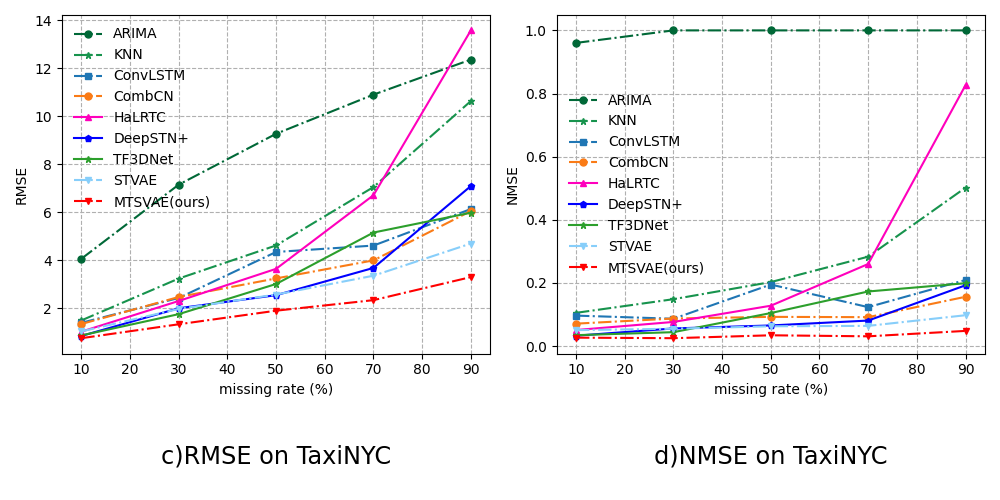
\includegraphics[width=\textwidth]{myplot_taxinyc.png}
\vspace{-1em}
\caption{填充效果图 \label{impute}}
\end{figure}

对于基于神经网络的方法,有ConvLSTM、DeepSTNPlus、CombCN和ST-VAE。前两个模型应用于交通数据的预测问题,其余模型用于交通数据的填充问题。在应用于交通数据预测问题的模型中,ConvLSTM将卷积操作集成到LSTM单元,使得它不仅能处理短期时间特征,还能处理长期时间特征,因而使它的性能优于HaLRTC。但遗憾的是,ConvLSTM模型仍然忽略了对全局特征的应用,这是限制它的实验效果进一步提升的一个重要因素。相比之下,MTSVAE可以捕获不完整交通数据的全局空间特征。

\begin{figure}[htbp] 
\centering
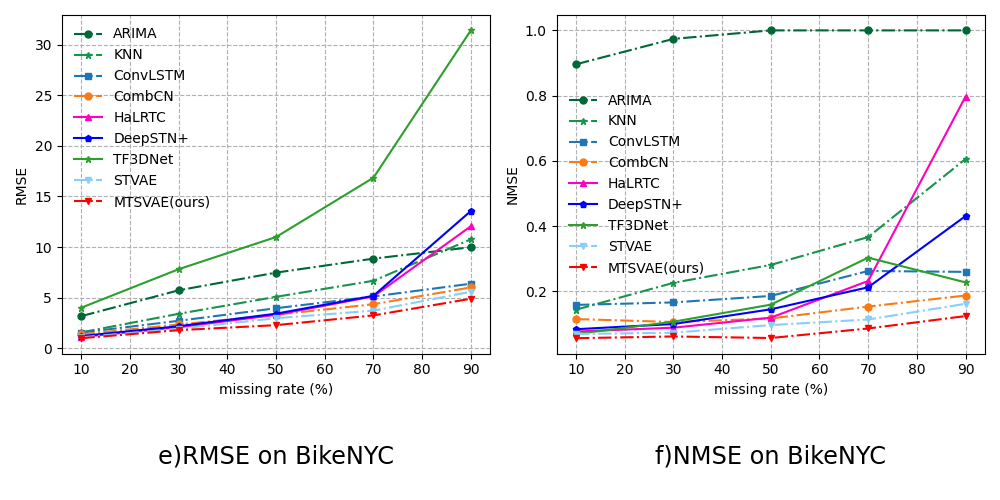
\includegraphics[width=\textwidth]{myplot_bikenyc.png}
\vspace{-1em}
\caption{填充效果图 \label{impute}}
\end{figure}

DeepSTNPlus是一个基于自动编码器的交通预测模型。DeepSTNPlus的两个重要组成构件是多层空间卷积模块,以及时间卷积模块。多层空间卷积模块可以帮助模型学习全局空间特征。时间卷积模块可以帮助模型学习时间特征。但是,DeepSTNPlus模型有一个很重要的缺陷就是,模型训练需要使用不带缺失值的训练数据集。相比之下,MTSVAE中的特征编码模块可以处理不完整的数据,这意味着可以通过使用不完整的交通数据训练模型MTSVAE。

在应用于交通数据填充问题的模型中,CombCN是基于自动编码器的模型,主要包含了3D卷积以及2D卷积。它使用3D卷积处理时间一致性问题,以及使用2D卷积提取空间特征。这些特点使得它可以有效处理视频填充问题。相比之下,MTSVAE使用BiconvGRUI提取有效时间特征,以及采用2D门控卷积学习有效空间特征。同时,MTSVAE是基于变分自编码器的模型,这意味着MTSVAE比那些基于自编码器的模型具有更强的鲁棒性。因此,MTSVAE比CombCN表现得更出色。

ST-VAE是一种类似的深度贝叶斯模型,它可以通过西尔维斯特标准化流变分编码提取不完整数据和潜在变量之间的随机映射。同时,它还可以通过3D卷积来学习时空特征。但遗憾的是,它忽略了不同的时间依赖关系的特性。相比之下,我们提出的模型MTSVAE可以学习不同时间依赖性的特征,这使得其性能优于ST-VAE。

\begin{table}[htbp] 
\caption{消融实验对比表(Mts:Multi temporal streams,FEm:Feature Encoding module)} 
\label{tb_ab} 
\vspace{0.5em}\centering\wuhao
\subtable[TaxiBJ数据集的RMSE / NMSE指标对比]{
\begin{tabular*}{\hsize}{@{}@{\extracolsep{\fill}}lccccc@{}}
%\begin{tabular}{lccccc}
\toprule[1.5pt]
缺失率 & 10\% & 30\% & 50\% & 70\% & 90\%\\
\midrule[1pt]
Single stream VAE         & 3.86/0.0280  & 7.15/0.0371  & 10.67/0.0417  & 12.44/0.0453  & 15.05/0.0449 \\
\textit{MTSVAE} w/o Mts  & 3.10/0.0183  & 5.92/0.0220  & 8.28/0.0253  & 10.41/0.0302  & 14.27/0.0379 \\
\textit{MTSVAE} w/o FEm   & 3.80/0.0278  & 7.00/0.0310  & 10.18/0.0382  & 12.77/0.0439  & 14.84/0.0428 \\
\textit{MTSVAE}           & \textbf{2.90}/\textbf{0.0160}  & \textbf{5.38}/\textbf{0.0183}  & \textbf{7.68}/\textbf{0.0215}  & \textbf{10.40}/\textbf{0.0290}  & \textbf{13.44}/\textbf{0.0359} \\
\bottomrule[1.5pt]
\end{tabular*}
}


%\subtable[TaxiNYC数据集下的消融实验对比表]{
%\begin{tabular}{ccccccccccc}
%\toprule[1.5pt]
%缺失率 &\multicolumn{2}{c}{10\%} & \multicolumn{2}{c}{30\%} & \multicolumn{2}{c}{50\%} & \multicolumn{2}{c}{70\%} & \multicolumn{2}{c}{90\%}\\
%& NMSE & RMSE & NMSE & RMSE & NMSE & RMSE & NMSE & RMSE & NMSE & RMSE \\
%\midrule[1pt]
%Pure-3DVAE      & 0.0358 (0.0002) & 4.34 (0.01) & 0.0406 (0.0003) & 8.01 (0.03)  & 0.0454 (0.0007) & 11.12 (0.08) & 0.0497 (0.0008) & 13.57 (0.10) & 0.0710 (0.0014) & 18.85 (0.18)\\
%STVAE w/o SNFs  & 0.0344 (0.0002) & 4.26 (0.01) & 0.0395 (0.0003) & 7.90 (0.03)  & 0.0432 (0.0003) & 10.83 (0.04) & 0.0474 (0.0008) & 13.25 (0.12) & 0.0505 (0.0007) & 15.93 (0.11)\\
%STVAE w/o DCB   & 0.0347 (0.0003) & 4.28 (0.02) & 0.0398 (0.0003) & 7.94 (0.03)  & 0.0410 (0.0004) & 10.64 (0.05) & 0.0477 (0.0006) & 13.29 (0.08) & 0.0536 (0.0009) & 16.39 (0.13)\\
%STVAE           & 0.0342 (0.0002) & 4.24 (0.01) & 0.0370 (0.0003) & 7.66 (0.04)  & 0.0408 (0.0003) & 10.53 (0.04) & 0.0454 (0.0004) & 12.96 (0.05) & 0.0497 (0.0004) & 15.80 (0.06)\\
%\bottomrule[1.5pt]
%\end{tabular}
%}
\subtable[TaxiNYC数据集的RMSE / NMSE指标对比]{
\begin{tabular*}{\hsize}{@{}@{\extracolsep{\fill}}lccccc@{}}
%\begin{tabular}{lccccc}
\toprule[1.5pt]
缺失率 & 10\% & 30\% & 50\% & 70\% & 90\%\\
\midrule[1pt]
Single stream VAE                & 0.86/0.0352  & 1,66/0.0393  & 2.17/0.0440  & 2.99/0.0522  & 4.41/0.0892 \\
\textit{MTSVAE} w/o Mts  & 0.88/0.0362  & 1.54/0.0338  & 2.05/0.0401  & 2.75/0.0429  & 4.90/0.1063 \\
\textit{MTSVAE} w/o FEm   & 0.75/0.0272  & 1.47/0.0345  & 2.14/0.0435  & 2.57/0.0409  & 3.21/0.0416 \\
\textit{MTSVAE} & \textbf{0.76}/\textbf{0.0269}  & \textbf{1.34}/\textbf{0.0252}  & \textbf{2.23}/\textbf{0.0469}  & \textbf{2.34}/\textbf{0.0311}   & \textbf{3.30}/\textbf{0.0483} \\
\bottomrule[1.5pt]
\end{tabular*}
}

\subtable[BikeNYC数据集的RMSE / NMSE指标对比]{
\begin{tabular*}{\hsize}{@{}@{\extracolsep{\fill}}lccccc@{}}
%\begin{tabular}{lccccc}
\toprule[1.5pt]
缺失率 & 10\% & 30\% & 50\% & 70\% & 90\%\\
\midrule[1pt]
Single stream VAE                & 1.02/0.0689  & 1.95/0.0806  & 3.08/0.1014  & 3.71/0.1133  & 6.28/0.274 \\
\textit{MTSVAE} w/o Mts  & 1.05/0.0647  & 1.96/0.0747  & 2.86/0.0879  & 3.29/0.100  & 5.72/0.1686 \\
\textit{MTSVAE} w/o FEm   & 0.96/0.0579  & 1.83/0.0706  & 2.96/0.0961  & 3.66/0.109  & 5.58/0.1614 \\
\textit{MTSVAE} & \textbf{0.99}/\textbf{0.0559}  & \textbf{1.78}/\textbf{0.0613}  & \textbf{2.28}/\textbf{0.0565}  & \textbf{3.24}/\textbf{0.0857}   & \textbf{4.89}/\textbf{0.1238} \\
\bottomrule[1.5pt]
\end{tabular*}
}
\end{table}
另外,本章还进行了消融实验以显示\textit{MTSVAE}中两个主要模块的效果:多时间流模块和特征编码模块。本章节重新配置\textit{MTSVAE}以创建如下所述的三个变体。 
1)单流\textit{VAE}:移除了多时间流、自注意力模块,并且仅在\textit{VAE}中使用了\textit{convGRU}以及多层普通\textit{2D}卷积。 

2)不含多时间流模块的\textit{MTSVAE}:删除多时间流模块,同时保留特征编码模块。 

3)不含特征编码模块的\textit{MTSVAE}:编码模块被\textit{convGRU}以及多层普通\textit{2D}卷积取代,同时保留了多时间流模块。 

表3-2展示了\textit{MTSVAE}以及它的三个变体在不同缺失率的实验数据集上的\textit{NMSE}和\textit{RMSE}的结果。如表3-2所示,\textit{MTSVAE}在两个评估指标上均优于其他三个变体,这一结果意味着编码模块对不完整交通数据的强大建模能力以及多时间流模块在对交通数据不同周期依赖性建模方面的有效性。

\section{本章小结} \label{sec3_6}
本章主要研究考虑时间缺失值分布特性的填充算法设计,通过将城市人群轨迹数据转换成视频流的方式,巧妙地把缺失值填充问题转换成张量填充问题。并且在其基础上设计了基于时空变分自编码器的多时间流缺失值填充算法,该算法通过添加Biconvgrui模块来提取带有缺失值的交通数据的时间分布特性,同时使用双自注意力机制来更为精确地提取存在值的时空特征,实验表明在面对较为复杂的数据集时表现突出。接着介绍了该模型损失函数以及缺失值填充,并给出了填充效果展示。最后,本章进行了多轮实验,实验结果证实了该模型的有效性。

% Local Variables:
% TeX-master: "../thesis"
% TeX-engine: xetex
% End: